\chapter{Implementácia}
\label{kap:imp}
V tejto kapitole popíšeme technológie, ktoré sme vybrali na implementáciu aplikácie. Ďalej popíšeme základné problémy, ktoré vznikli pri spracovaní dát, pri implementácii dátovej štruktúry a navrhovaného algoritmu. Ukážkami kódov priblížime, ako sme tieto problémy riešili. 

\section{Technológie}
Serverovú časť aplikácie sme implementovali v jazyku \textit{Java}, konkrétne vo verzii \textit{Java 11} s využitím frameworku \textit{SpringBoot}. Na mapovanie \textit{Java} objektov na databázové entity sme použili ORM framework \textit{Hibernate}. Pre komunikáciu s frontendom sme si vybrali REST architektúru. Táto architektúra je dokumentovaná pomocou technológie \textit{Swagger}. Na frontendovej strane sme si zvolili progresívnu webovú aplikáciu a na jej implementáciu sme použili moderný JavaScriptový framework \textit{Vue.js}, konkrétne verziu \textit{Vue 2}. Zároveň sme použili knižnicu \textit{Vuex} na spravovanie stavu aplikácie. 

\section{Dáta}
\subsection{Parsovanie dát zo súboru}
\label{sec:parsing}
\subsubsection{Dáta statických cestovných poriadkov}
Náš projekt obsahuje dáta vo formáte GTFS (\ref{sec:gtfs}), ktoré reprezentujú cestovné poriadky v bratislavskej MHD platné pre obdobie v minulosti. 
Dáta zo súboru \textit{stops.txt} sme zachytili v troch rôznych objektoch. Polohu zastávky sme vyčlenili do zvlášť objektu \textit{Coords}. Zastávky s rovnakým názvom sme zoskupili do objektu \textit{StopArea}. Samotný objekt \textit{Stop} zachytáva zónu a informáciu o tom, či je zastávka na znamenie. 

Keďže v dátach nemáme informáciu o peších presunoch medzi jednotlivými zastávkami, implementovali sme \textit{FootPathsFileGenerator}. Táto služba nám využitím \textit{Google Distance Matrix API} zistí vzdialenosti medzi jednotlivými zastávkami a vytvorí súbor \textit{foot\_paths.txt}. Súbor obsahuje len také dvojice zastávok, ktoré sme definovali v sekcii \ref{sec:foot-paths}. Dáta z tohto súboru sú v namapované na objekty \textit{FootPath}. 

Každý dátum z rozmedzia dátumov platnosti daného cestovného poriadku potrebujeme zaradiť do pod nejaký typ dňa (pracovné dni, víkendy, školské prázdniny, štátne sviatky,...). Z dát uložených v  GTFS štandarde sa komplikovaným spôsobom zisťuje, ktoré typy dní prislúchajú konkrétnemu dátumu. Objekty \textit{CalendarDate} budú uchovávať dátumy z rozmedzia dátumov platnosti cestovného poriadku. V objektoch \textit{ServiceDay} budú uložené jednotlivé typy dní. 

Dáta zo súborov \textit{trips.txt}, \textit{routes.txt} a \textit{stop\_times.txt} len mapujeme na objekty \textit{Trip}, \textit{Route} a \textit{StopTime}. Zmenou je, že informáciu o tom, či je zastávka na znamenie si neudržujeme v objekte \textit{StopTime}, ale priamo v objekte \textit{Stop}. V dátach chýbala informácia o tom, či je jazda linky vedená nízkopodlažným vozidlom. Parameter \textit{lowFloor} náhodne generujeme pre jednotlivé jazdy do objektu \textit{Trip}.

\subsubsection{Dáta o meškaní vozidiel}
V projekte máme aj dáta o meškaniach vozidiel. Ich formát sme spomínali v \ref{sec:delay-data}. Potrebujeme aby sa každú minútu prečítali tie dáta ktoré patria k aktuálnemu dňu a vznikli v predchádzahjúcej minúte. Použili sme springovskú anotáciu \textit{@Scheduled} s parametrom \textit{fixedRate=60000}, ktorá zaručí, že každú minútu sa bude vykonávať funkcia, ktorá s súbore hľadá záznamy o meškaní z predchádzajúcej minúty. Vyfiltrujú sa tie záznamy, ktoré majú zápornú hodnotu meškania a snažíme sa nájsť jazdu, ktorej tieto údaje prislúchajú. Zaujímavé údaje sú zastávka $p$, linka $r$, čas záznamu $t$ a meškanie $d$. Ak nájdeme v linke $r$ jazdu, ktorá stojí na zastávke v čase $t-d$, nastavíme jej hodnotu meškania $d$ v dátovej štruktúre, ako aj zastávke $p$ a všetkým  nasledujúcim za ňou.

\subsection{Použitie databázy}
V projekte sme sa rozhodli použiť relačná \textit{SQL} databázu na uchovanie všetkých dát a vzťahov, ktoré vytvárame a vkladáme pri prvotnom spustení aplikácie. Pôvodne sme plánovali z databázy vytvárať dátovú štruktúru pre algoritmus, keďže v databáze sú zachytené vzťahy medzi dátami.

Počas implementácie sme však zistili, že voľba ORM framework \textit{Hibernate} nebola veľmi dobrou voľbou. Mysleli sme si, že \textit{Hibernate} bude postačujúci pre jednorazové vloženie údajov do databázy a následne pre jednoduché čítanie údajov bez nutnosti použitia komplikovaných \textit{SQL} príkazov. Vzťahy medzi údajmi sú však komplexné a údajov je veľké množstvo. Najväčšiu záťaž sme pocítili pri čítaní všetkých údajov z tabuľky trips, ktorá je prepojená so všetkými ostatnými tabuľkami. Tieto údaje však potrebujeme na vytvorenie dátovej štruktúry. Z toho dôvodu sme sa rozhodli, že z databázy budeme ťahať údaje pre frontend. Napríklad na zobrazenie všetkých liniek a zastávok, an ktorých stoja. Ďalej na zobrazenie všetkých zastávok spolu so súradnicami pre možnosť vyberania zastávky z mapy alebo všetky skupiny zastávok pre vyberanie zastávky zo zoznamu.

\subsection{Testovacie dáta}
Dátová sada vo formáte GTFS obsahuje veľa záznamov. Už pri implementácii bolo potrebné myslieť na to, ako budeme overovať správnosť mapovania dát do databázy, korektnosť vytvorenej dátovej štruktúry a v neposlednom rade vedieť ohodnotiť a upraviť algoritmus tak, aby počítal čo najoptimálnejšie cesty. Pri veľkej dátovej sade sa ťažko testuje správnosť implementácie a preto sme pred samotnou implementáciou navrhli zmenšenú testovaciu sadu dát. 
Táto sada obsahuje 7 skupín zastávok (\textit{stopArea}), 16 zastávok, 3 linky, 70 jázd a 185 záznamov \textit{stopTimes}. Pre porovnanie reálna sada obsahuje až vyše 700 000 \textit{stopTimes}. Okrem GTFS dát sme vytvorili aj pár testovacích záznamov o meškaní. 

Pre jednoduché prepínanie medzi dvomi dátovými sadami aplikácie sme použili profily z frameworku \textit{Spring}. Každý profil má definované premenné prostredia, ktoré pre náš projekt definujú napríklad údaje pre dátové pripojenie ako názov databázy, používateľa a heslo do databázy. Ďalej sú to cesty k GTFS súborom a dátam o meškaniach. 

\section{Dátová štruktúra}
Dátová štruktúra sa vytvára pri spustení serverovej aplikácie. Najskôr sme začali implementovať vytvorenie dátovej štruktúry podľa návrhu, teda ťahaním údajov z databázy. Z dôvodu pomalého ťahania údajov z databázy sme sa rozhodli obísť databázu a dátovú štruktúru vytvárame hneď pri parsovaní súboru. Tento proces trvá približne 5 -7 minút v závislosti od zariadenia. Toto trvanie je prijateľné pri produkcii keďže aplikácia sa bude spúšťať len pri aktualizácii cestovných poriadkoch a v prípade nejakých výpadkov. V procese implementácie je však 7 minútové čakanie veľmi obmedzujúce pri každom spustení aplikácie. Vytvorený a naplnený model sme sa rozhodli serializovať do súboru. Proces deserializácia už trval do jednej minúty. 

Premýšľali sme aj o umiestnení dátovej štruktúry a algoritmu na klientskej strane. Toto riešenie by umožňovalo používateľovi vyhľadávať aj offline, kedy by aplikácia nevyhľadávala s prihliadnutím na meškanie vozidile. Otázkou je, kedy by sa dátová štruktúra vytvárala. Ak by sa vytvárala len pri prvotnej inštalácii alebo po aktualizácii cestovných poriadkov dátová štruktúra by zaberala veľa pamäte. Serializovaný model dátovej štruktúry má takmer 0,5 GB. Druhá možnosť je načítavať dátovú štruktúru pri každom spustení aplikácie, čo by mohlo trvať neprimerane dlho. Síce sú frontendové jazyky rýchlejšie a objekty sú menšie, stále by mohol byť problém s vytvorením dátovej štruktúry a pamäťou, ktorá aplikácia zaberá. Zostávame teda pri vyhľadávaní spojov a udržiavaní dátovej štruktúry na serverovej strane ako aj mnohé existujúce aplikácie.

\subsection{Implementácia dátovej štruktúry}
Pre celý beh aplikácie bude potrebná len jedna inštancia dátovej štruktúry. Pri spustení aplikácie sa vytvorí aplikačný kontext, ktorý reprezentuje množinu prepojených komponentov. Tieto komponenty manažuje \textit{IoC kontainer}. Objekt \textit{DataStructure} je označený anotáciou \textit{@Component}, ktorý pri autowirovaní vytvorí \textit{DataStructureModel} načítaním z GTFS dát v produkčnom prostredí alebo deserializovaním zo súboru v implementačnej fáze.\textit{ @Component }je vlastne \textit{@Bean} a ten sa v \textit{Springu} správa ako \textit{Singleton}. 
Trieda \textit{DataStrctureModel} definuje model dátovej štruktúry pre RAPTOR algoritmus, ktorá je tvorená šiestimi dátovými štruktúrami. 
\begin{lstlisting}
public class DataStructureModel implements Serializable {
    private Map<Route, List<Subroute>> routeSubroutes;
    private Map<Long, List<Transfer>> stopTransfers);
    private Map<Stop, List<String>> stopSubroutes;
    private Map<String, Subroute> subroutesByIndex;
    private Map<String, Map<Long, Integer>> stopIndexInSubroute;
    private List<CalendarDate> calendarDates;
}
\end{lstlisting}
Štruktúra \textit{routeSubroutes} je definovaná slovníkom, kde kľúčom je linka $r$ a hodnota je pole úsekov, ktoré patria linke $r$. 

Kľúčom v \textit{stopTransfers} je identifikačné číslo zastávky $p$ a hodnotou je pole peších prestupov, pričom začiatočná zastávka je zastávka $p$. 

Slovník \textit{stopSubroutes} ma zastávku $p$ ako kľúč a hodnotou je pole indexov úsekov linky, ktoré stoja na zastávke $p$. Index úseku linky je textový reťazec, pretože má formát \{identifikačé číslo linky\}\_\{číslo úseku v rámci linky\}. Tento index sa vytvára pri vytváraní dátovej štruktúry, ako aj celý objekt \textit{Subroute}. 

Slovník \textit{subroutesByIndex} obsahuje zoznam všetkých úsekov liniek, s tým že je indexovaný podľa unikátneho reťazca.

Štruktúra \textit{stopIndexInSubroute} poskytuje poradové číslo zastávky v rámci úseku linky. Posledné je pole objektov \textit{CalendarDate}, ktoré poskytuje  všetky dátumy z rozsahu platnosti cestovných poriadkov a ku každému dátumu $d$ je priradená množina typov dní. 

\subsection{Naplnenie dátovej štruktúry}
Pri plnení dátovej štruktúry sa zavolá \textit{LoadService}, ktorý parsuje dáta zo súborov GTFS do polí objektov \textit{StopArea}, \textit{Stop}, \textit{Coords}, \textit{Trip}, \textit{Route}, \textit{CalendarDate}, \textit{ServiceDay}, \textit{FootPath}, \textit{StopTime}. Tieto objekty sa navzájom na seba odkazujú. Ako sme spomínali v sekcii \ref{sec:parsing}, tieto polia nie sú len kópiou GTFS dát, ale obsahujú nejaké zmeny. Napríklad zoskupenie zastávok s rovnakým menom do objektu \textit{StopArea} alebo súradnice do objektov \textit{Coords} a pod.. Pri vytváraní dátovej štruktúry z polí objektov ešte navyše zoskupujeme jazdy s rovnakou postupnosťou zastávok do úsekov linky \textit{Subroute}. 

Ako sme už spomínali na začiatku, dátovú štruktúru po naplnení dátami serializujeme, aby sme neboli pri implementácii obmedzovaný časom spustenia aplikácie. Objekty v dátovej štruktúre sa však na seba odkazujú cyklicky a preto je potrebné cyklické referencie pri plnení dátovej štruktúry odstrániť. 

\section{Časový simulátor}
Keďže máme k dispozícii historické dáta o meškaní vozidiel a platnosť cestovných poriadkov je tiež v minulosti, potrebujeme v aplikácii simulovať čas v minulosti. V konfigurácii nastavujeme čas, ktorý, aplikácia začína spustením. Na prelome dňa sa čas vynuluje a navýši sa dátum o jeden deň. 
Pri spustení klienta sa klient dopytuje na aktuálny čas servera. Klientská strana pokračuje v navyšovaní času po sekunde rovnako ako serverová strana. Klient potrebuje mať stále aktuálny čas, aby vedel obmedziť vyhľadávanie do minulosti. Keďže pracujeme s reálnymi dátam, pri vyhľadávaní do minulosti by mohol nastať problém. 

Pri prvotnom spustení serverovej strany zároveň aktualizujeme dátovú štruktúru dátami o meškaní. Podľa aktuálneho dňa vyhľadáme súbor, ktorý obsahuje meškania. Zo súboru vytiahneme všetky záznamy od začiatku dňa po aktuálny čas. Podľa získaných záznamov nastavíme meškajúcim linkám hodnotu meškania v dátovej štruktúre. S každou nasledujúcou pribudnutou minútou hľadáme už len také záznamy, ktoré vznikli v predchádzajúcej minúte. 
Získané hodnoty meškania v minútach priradzujeme k získanej zastávke a ku všetkým zastávkam nasledujúcim za ňou. 

\subsection{Vlastná trieda \textit{Time}}
Na serverovej strane sme si vytvorili vlastnú triedu \textit{Time}, keďže s časom potrebujeme často pracovať nezávisle od dátumu. Jej parametrami sú: \textit{hours}, \textit{minutes}, \textit{seconds}, \textit{nextDay} a \textit{prevDay}. Trieda umožňuje skonštruovať čas z textového reťazca. Takto definovaný čas prichádza z GTFS dát, ktorý určuje kedy konkrétna jazda linky stojí na zastávke. Triedu čas vieme skonštruovať aj priamo kombináciou vymenovaných parametrov. Rovnako vieme skonštruovať maximálny čas t=23:59:59, ktorý potrebujeme definovať pri inicializácii výsledkov RAPTOR algoritmu. Časy vieme medzi sebou porovnávať alebo k nim odpočítavať a pripočítavať minúty.

Parameter \textit{nextDay} slúži na porovnávanie časov, keďže v dátach sa vyskytujú aj časy nad 23:59. Metóda porovnávania časov prihliada aj na parameter nextDay. Tento parameter navyšujeme aj vtedy, keď pri pripočítavaní minút k času presiahneme maximálny čas.
Parameter \textit{prevDay} používame pri hľadaní jazdy v dátovej štruktúre podľa záznamov o meškaní vozidiel. Ak  máme záznam v čase t=0:00 a vozidlo mešká $1$ minútu, od času $t$ je potrebné odpočítať $1$ minútu. Dostávame sa tak do predchádzajúceho dňa, kde je potrebné hľadať prislúchajúcu cestu. 

\section{RAPTOR Algoritmus}

\subsection{Výsledky RAPTOR algoritmu}
RAPTOR algoritmus operuje v kolách a v každom kole vylepšuje časy zastávkam. Potrebujeme si pre každé kolo držať pole zastávok. Pre každú zastávku a každé kolo existuje jeden najlepší čas. Tento čas si budeme držať v slovníku roundArrivals, ktoré je definované:
\begin{lstlisting}
private Map<Integer, List<StopArrivalTime>> roundArrivals; 
\end{lstlisting}
Kľúčom je kolo a jeho hodnotou je pole objektov \textit{StopArrivalTime}. Tento objekt zjednocuje zastávku a čas príchodu na zastávku. Pri vyhodnocovaní však budeme potrebovať hľadať podľa zastávky najlepší čas a preto si udržujeme ešte jeden slovník, ktorý je definovaný:
\begin{lstlisting}
private Map<Stop, TimeRound> bestArrivals;
\end{lstlisting}
Aby sme po zbehnutí algoritmu vedeli vytvoriť cesty z výsledkov, potrebujeme si pamätať, ako sme pre zastávku získali  vylepšený čas v každom kole. Definovali sme slovník \textit{roundActions}.
\begin{lstlisting}
private Map<Stop, List<RoundTimeAction>> roundActions;
\end{lstlisting}
Slovník pre každú zastávku udržuje pole objektov \textit{RoundTimeAction}. Tento objekt je tvorený indexom kola, časom a objektom \textit{Action}. Objekt \textit{Action} je určený dvomi zástavkami a typom akcie, čo môže byť buď peší presun alebo úsek jazdy. V prípade pešieho presunu si pamätáme, aké je jeho trvanie a v prípade úseku jazdy si pamätáme identifikačné číslo jazdy. Pre konkrétnu zastávku a kolo môže existovať viac akcií, keďže najlepší čas môžeme dosiahnuť dvomi rôznymi akciami. Pred vytváraním ciest tieto akcie ešte prefiltrujeme. Môžu totiž existovať také 2 akcie, že zastávku sme dosiahli čas 6:00 v kole $2$ a zároveň sme tento čas dosiahli v kole $3$. Druhá akcia je nevýhodnejší takže je môžeme odfiltrovať ešte pred vytváraním ciest.

Z takto vyfiltrovaných akcií tvoríme rekurzívne cesty s tým, že začíname v konečnej zastávke  a končíme, ak sme dosiahli niektorú zo začiatočných zastávok. V prípade, že vyhľadávanie začínalo v aktuálnej lokalite, pripojíme k ceste na začiatok ešte prvotný peší presun z aktuálnej lokality do začiatočnej zastávky.

\subsubsection{Target prunning}
Do výsledkov RAPTOR algoritmu sme pridali ešte jeden slovník, ktorý uchováva pre každú skupinu zastávok (\textit{stopArea}) najlepší čas pre každé kolo. 
\begin{lstlisting}
private Map<StopArea, TimeRound> stopAreaBestArrivals;
\end{lstlisting}
Týmto znížime počet označených zastávok a rovnako aj výpočtový čas. Keďže my hľadáme cesty z jednej \textit{stopArea} do druhej \textit{stopArea} a nie medzi zastávkami, vieme obmedziť prehľadávanie. Ak sme sa už do niektorej zo zastávok v spoločnej \textit{stopArea} dostali skorej, čas nevylepšíme a zastávku neoznačíme ako prestupné miesto na ďalšie prehľadávanie. 

\subsection{Hľadanie najbližšej vyhovujúcej jazdy}
\label{trip-finding}
RAPTOR algoritmus funguje tak, že hľadáme najskoršiu vyhovujúcu jazdu linky $r$ po čase $\tau$, ktorá stojí na zastávke $p$ a jazdí v niektorý zo zadaných typov dní ($ServiceDay$). V algoritme nepracujeme s linkami, ale s objektami \textit{Subroute}. Tento objekt obsahuje slovník, ktorý je indexovaný objektom \textit{ServiceDay} a hodnotou je pole jázd (\textit{SubrouteTrip}). Tým pádom jazdu nehľadáme vo všetkých jazdách, ktoré patria linke, ale len v takých, ktoré stoja na zastávke $p$ v niektorý požadovaných typov dní. 

Aby sme nemuseli prechádzať všetky jazdy v linke, hľadanie jazdy funguje tak, že začíname od poslednej jazdy v utriedenom poli. Spoliehame sa, že jazdy sú utriedené podľa času príchodu na prvú zastávku vzostupne. Kým nie je čas príchodu jazdy na zastávku $p$ menší ako $\tau$, iterujeme jazdy smerom na začiatok poľa a do premennej \textit{lastTrip} si ukladáme vždy aktuálnu jazdu. V momente keď narazíme na jazdu, ktorá na zastávke $p$ stojí skôr ako je čas $\tau$, máme v premennej \textit{lastTrip} vyhovujúcu jazdu. Index tejto jazdy si uložíme do poľa \textit{foundTripsIndices} v prípade, že by sme pre túto \textit{subroute} potrebovali nájsť ešte nejakú skoršiu jazdu v ďalšom hľadaní. Túto optimalizáciu môžme spraviť, keďže jazdy, ktoré prídu na zastávku neskôr ako označená jazda, nás už nezaujímajú.  

Môže nastať prípad, že všetky jazdy stoja na zastávke $p$ skôr ako v čase $\tau$, preto sme museli pridať podmienku, ktorá overí, či príchod poslednej jazdy na zastávku $p$ je neskôr ako čas $\tau$. Ak nie je, nevrátime žiadnu cestu. 

Časť implementácie vyhľadávania najbližšej vhodnej jazdy môžeme vidieť v ukážke kódu: 
\begin{lstlisting}
if (arrivalTimeOfLastTripEarlierThanSearchedTime(subrouteTrips, searchedTime, stopIndex)) { return null;}
for (int i = this.foundTripsIndices.get(subrouteServiceDay); i >= 0; i--) {
 SubrouteTrip trip = subrouteTrips.get(i);
 Time tripStopTime = trip.getStopTimeObjects()[stopIndex].getTime();
 if (!onlyLowFloor || trip.isLowFloor()) {
  if (tripStopTime.isBefore(searchedTime)) { break; }
  else { lastFound = trip; }
  foundTripsIndices.put(subrouteServiceDay, i);
 }
}
\end{lstlisting}

\subsubsection{Zoradenie jázd v rámci linky}
Už pri vytváraní dátovej štruktúry sme riešili ako správne zotriediť jazdy v linke. Najskôr sme sa rozhodli využiť atribút \textit{sequence order}, ktorý je priradený ku každému objektu \textit{StopTime}. \textit{StopTime} okrem iného definuje v akom čase stojí jazda linky na zastávke. Atribút \textit{sequence order} by mal určiť poradie zastávky v rámci jazdy a zároveň aj v rámci celého dňa. Prvá jazda linky na prvej zastávke má sequence order $1$ a toto číslo sa navyšuje až po poslednú zastávku poslednej jazdy linky. Vieme teda vypočítať poradie jazdy v linke. 

Stále sme však prichádzali na problém, že linky nie sú zoradené správne. Naimplementovali sme sližbu, ktorá nám vyvorí csv súbor s čitateľným cestovním poriadkom. Po hlbšom skúmaní sme zistili, že atribút \textit{sequence order} nezoraďuje jazdy linky tak, ako by sme to potrebovali pre náš algoritmus. Zároveň sme zistili, že časy príchodu jazdy na zastávku sú v niektorých prípadoch väčšie ako čas 23:59:59. Dokonca existujú také jazdy, ktoré prichádzajú na všetky zastávky linky až na druhý deň ako môžme vidieť na obrázku \ref{fig:weird-times}.

\begin{figure}[H]
\centerline{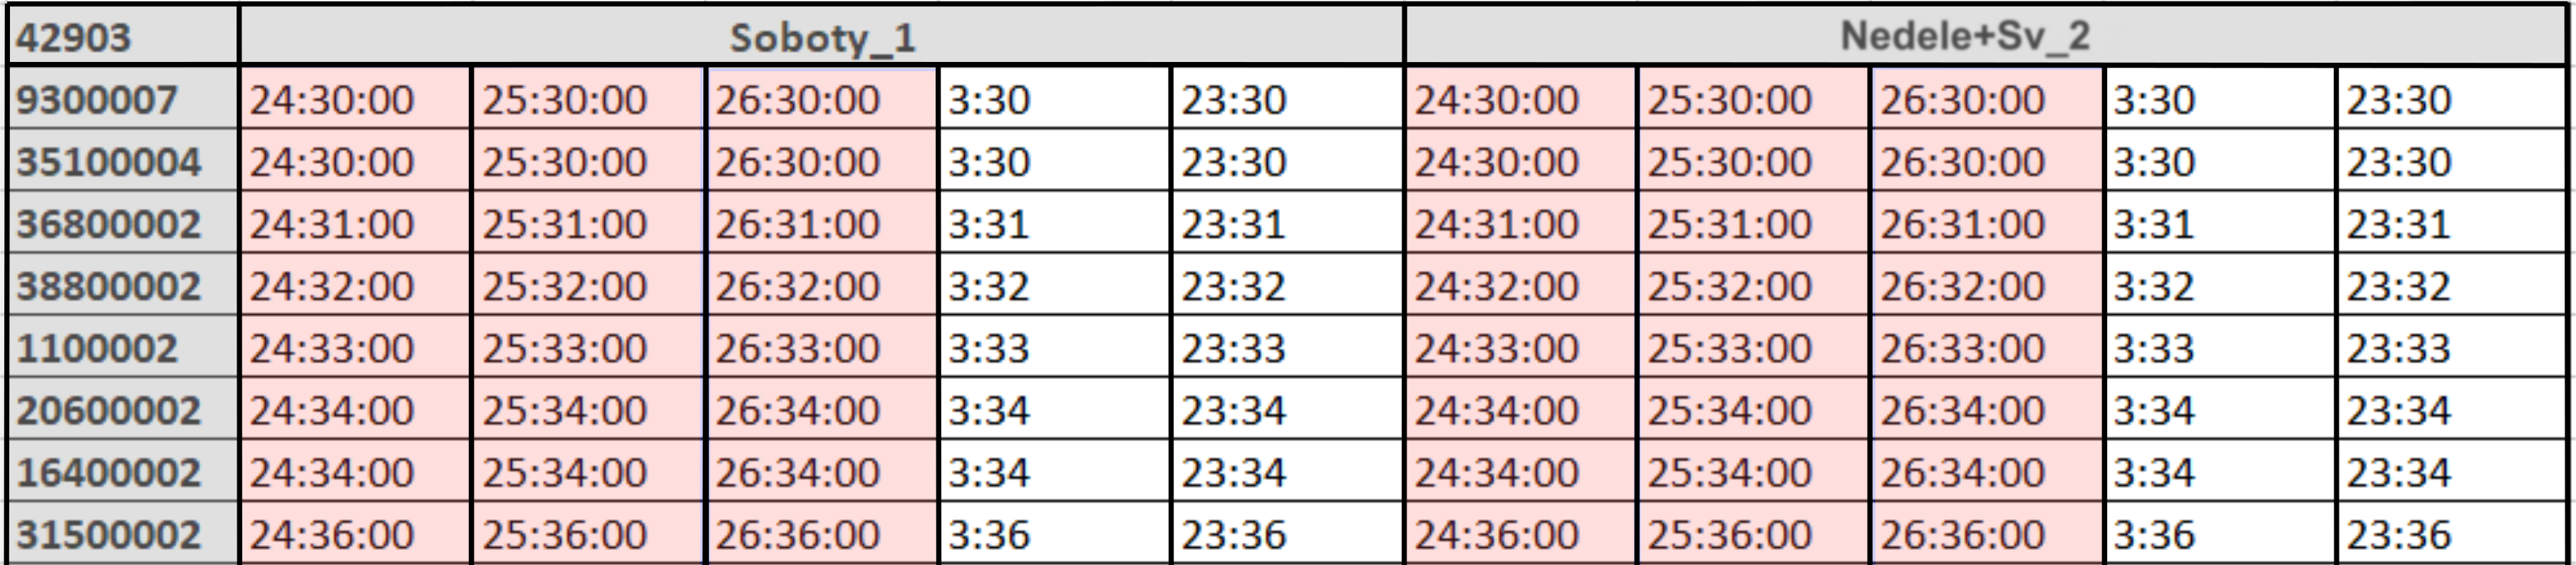
\includegraphics[width=1\textwidth]{images/weird-times}}
\caption[Ukážka exportovaného cestovného poriadku]{Ukážka exportovaného cestovného poriadku}
\label{fig:weird-times}
\end{figure} 

Tieto výnimky v dátach nám po menšej analýze nedávali zmysel a keďže sme boli už v pokročilej fáze vývoja algoritmu, rozhodli sme sa takéto dáta odignorovať. Z toho dôvodu vyhľadávanie na prelome dní nemusí fungovať správne.

V každom prípade potrebujeme mať zoradené jazdy linky tak, aby vyhovovali nášmu algoritmu a teda podľa času príchodu na jednotlivé zastávky jazdy linky. Jazdy sa udržujú v štruktúre \textit{stopSubroutes}, kde pre každú zastávku $p$ existuje pole indexov \textit{subroutes}, ktoré na zastávke $p$ operujú. \textit{Subroute} je zoskupenie jázd s rovnakou postupnosťou zastávok v rámci linky. Subroute si udržuje pole jázd indexovaných identifikačné čísloom \textit{serviceDay}, v ktorý táto jazda operuje. Toto pole jázd je zoradené podľa času príchodu jazdy na zastávku. 

\subsubsection{Prihliadanie na meškanie vozidiel}
Dostávame sa k jadru našej práce a prispôsobeniu algoritmu, aby prihliadal na dáta o meškaní. Ako sme už spomínali, na pozadí beží služba, ktorá zabezpečuje, že v dátovej štruktúre je pre každý \textit{StopTimeObject} správna hodnota parametra \textit{delay} pre aktuálny deň a aktuálny čas. 
Konkrétne dáta vkladáme do štruktúry \textit{stopSubroutes}, obsahujúcej aj objekty \textit{StopTimeObject}, ktoré si pre každú zastávku na každej jazde držia čas, kedy jazdy linky stojí na zastávke (\textit{time}) a zároveň, s akým predpokladaným omeškaním príde jazdy linky na zastávku (\textit{delay}). 

V dátovej štruktúre sa spoliehame že jazdy sú utriedené podľa času príchodu na zastávku. Pri vyhľadávaní v aktuálny deň budeme prihliadať aj na meškania. Čo znemená, že čas príchodu na zastávku predstavuje čas príchodu jazdy na zastávku podľa statických cestovných poriadkov + predpokladané meškanie jazdy na zastávku. Keďže každá jazda môže mať iné meškanie a môže nastať taká situácia, že jazda $t_1$ ma príchod na zastávku $p_1$ v čase 15:05 ale má meškanie $d_1=10$ minút. Predpokladaný príchod jazdy $t_1$ na zastávku $p_1$ je teda 15:15. Za ňou nasledujúca jazda $t_2$ má na zastávku $p_1$ prísť 15:10 a nemá zistené žiadne meškanie. V prípade, že by používateľ zadal vyhľadávanie v aktuálny deň napríklad o $\tau$ = 14:59 zo zastávky $p_1$, algoritmus by vybral jazdu $t_2$ ako najskoršiu jazdu, ktorú vie používateľ chytiť na zastávke $p_1$. Správnym riešením by však bolo vybrať jazdu $t_0$. Ilustráciu tejto situácie môžeme vidieť na obrázku \ref{fig:shedule-delays}. 

\begin{figure}[H]
\centerline{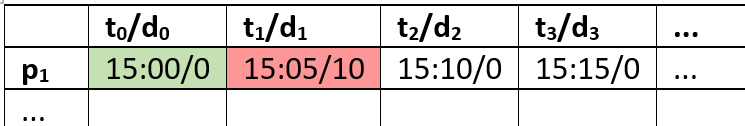
\includegraphics[width=0.6\textwidth]{images/shedule-delays}}
\caption[Hľadanie najbližšej jazdy s prihliadnutím na meškanie]{Hľadanie najbližšej jazdy s prihliadnutím na meškanie}
\label{fig:shedule-delays}
\end{figure} 

Pri hľadaní najbližšej jazdy teda zvažujeme dve rôzne situácie. V prípade, že vyhľadávame v iný deň ako v aktuálny deň, hľadáme jazdu tak ako sme spomínali na začiatku sekcie. Ak hľadáme v aktuálny deň, prechádzame cez všetky jazdy linky, kým nenájdeme takú jazdu $t$, pre ktorú platí:
$stopTime(t, p).time + stopTime(t, p).delay \geq \tau$ a zároveň je tento čas najmenší možný.

\subsection{Zapracovanie používateľských preferencií}
\subsubsection{Maximálny počet prestupov}
RAPTOR algoritmus končí vtedy, ak už neexistujú žiadne ďalšie označené zastávky, teda ak sa v predchádzajúcom kole nevylepšil žiadny z časov. RAPTOR algoritmus beží v kolách. Prvé kolo znamená 0 prestupov, druhé kolo 1 prestup, atď. Aby bol algoritmus obmedzený počtom prestupov, stačí pridať podmienku a obmedziť algoritmus navyše maximálnym počtom kôl. V kóde je táto podmienka umiestnená na začiatku vyhľadávania:
\begin{lstlisting} 
public RaptorResults search(SearchParams searchParams) {
 Set<Stop> markedStops = initializeMarkedStops(searchParams);
 RaptorResults raptorResults = initializeRaptorResults(searchParams);
 while(markedStops.size() > 0 && 
       raptorResults.getRound() <= searchParams.getMaxNumberOfTransfers()){        
  ...
 }
 return raptorResults;
}
\end{lstlisting}

\subsubsection{Maximálny čas pešieho presunu}
Pri prechádzaní zastávok, ktoré boli v predchádzajúcom kole vylepšené hľadáme pešie presuny do okolitých zastávok. Okolité zastávky boli pre každú zastávku radiálne vyhľadané v okolí $x$ metrov pri parsovaní dát. V algoritme hľadáme pre zastávku len také pešie presuny do iných zastávok, ktorých trvanie je menšie alebo rovné ako používateľom definovaný maximálny čas pešieho presunu. Umiestnenie v kóde:
\begin{lstlisting}
private void traverseTransfers(Set<Stop> markedStops, int maxTimeOfWalking){
 for(Transfer transfer: transfers){
  if(transfer.getDuration() <= maxTimeOfWalking) { ... }
 }
}
\end{lstlisting}
V algoritme však môže nastať prípad, vo viacerých kolách po sebe bude vybratý peší presun a v súčte trvanie týchto peších presunov môže trvať dlhšie ako používateľom definovaný maximálny čas pešieho presunu.
Takúto cestu neponúkneme používateľovi a vyfiltrujeme ju pred tvorením zoznamu výsledných ciest.

\subsubsection{Minimálny čas na prestup}
Nech nastane prípad, že na zastávke $A$ vystúpime v čase 6:00 a hodnota minimálneho času na prestup sú $2$ minúty. Nech jazda $t_1$ stojí na zastávke $A$ v čase 6:00 a jazda $t_2$ v čase 6:05. Hľadáme najskoršiu jazdu linky $r$, ktorú vieme stihnúť na zastávke $A$. Správnym riešením je jazdu $t_2$, nie jazdu $t_1$.

V prípade, že sa jedná o prvú akciu v ceste, nechceme pripočítavať minimálny čas na prestup. Pri prvom vyberaní jazdy ešte neprestupujeme. Začiatočný čas, teda nastavíme podľa kola, v ktorom sa algoritmus práve nachádza. V ukážke je ukízené ako získavame čas $\tau$, ktorý následne posielame do triedy \textit{TripFinder}, ktorá nám vráti najskorsšiu vyhovujúcu jazdu po čase $\tau$.
\begin{lstlisting}
private Time getStartingTime(RaptorResults raptorResults, int minTimeForTransfer, Time arrivalTime) {
 return raptorResults.getRound() == 1
        ? arrivalTime
        : new Time(arrivalTime).addMinutes(minTimeForTransfer);
}
\end{lstlisting} 

\subsubsection{Vyfiltrovanie len nízkopodlažných vozidiel}
Informáciu o nízkopodlažných vozidlách sme nedostali v dátach statických cestovných poriadkoch. Vygenerovali sme si ich náhodne pri importovaní dát a teda každá jazda linky má priradenú informáciu o type vozidla.
V kóde v sekcii \label{sec:trip-finding} môžeme vidieť podmienku, ktorá zabezpečí, aby v prípade nastavenia vyfiltrovania len nízkopodlažných spojov, algoritmus hľadal len také jazdy, ktoré obsluhujú nízkopodlažné vozidlá.

\section{Klientská strana} 
%V tejto sekcii popíšeme ako je aplikácia implementovaná na klientskej strane a popíšeme ako sme sa vysporiadali s časom v minulosti. Ďalej objasníme ako sme riešili zobrazenie zastávok v mape, zobrazenie časov vyhľadaných ciest alebo dopytovanie na nasledujúce cesty. 


\subsection{Implementácia klientskej strany} 
Pri navrhovaní funkcionalít aplikácie sme si načrtli obrazovky, podľa ktorých sme postupovali pri implementácii. 
Aplikáciu z pohľadu klienta tvoria 4 podstránky: hlavné menu, zoznam liniek, vyhľadávanie spojov a výsledky vyhľadávania. Hoci existujú rôzne knižnice znovu použiteľných komponentov, nenašli sme také, ktoré by vyhovovali našim požiadavkám. Vytvorili sme si preto vlastné komponenty napríklad komponent $Card.vue, Loader.vue$ alebo $Preferences.vue$. Tento komponent sa správa ako vysúvacia lišta, ktorá zobrazí možnosť navolenia vyhľadávacích parametrov. Údaje, ktoré sú zdieľané medzi podstránkami a komponentami sú uložené vo $vuex store$. História vyhľadávania sa ukladá do lokálneho úložiska prehliadača, aby aplikácia mohla ponúknuť používateľovi posledné parametre vyhľadávania.


\subsection{Dátum s čas}
Na klientskej strane sa potrebujeme tiež vysporiadať s časom v minulosti. Keďže chceme, aby aplikácia bola používateľsky prívetivá, predvolíme pri vyhľadávaní aktuálny dátum a čas. Na serverovej strane sa simuluje aktuálny dátum a čas a po spustení aplikácie na klientskej strane sa dotiahne zo servera aktuálny simulovaný dátum a čas. Klientská strana pokračuje v simulovaní času. 

Na výber dátumu sme použili komponent \textit{datepicker}. Tento komponent umožňuje nastaviť predvolený dátum a znemožniť výber dátumov v simulovanej minulosti. Ukážka komponentu je na obrázku \ref{fig:date-picker}.

Na zvolenie času sa si vytvorili vlastný komponent \textit{timepicker}, pretože žiadny z dostupných komponentov nespĺňal naše požiadavky. Náš komponent na výber času predvolí aktuálny simulovaný čas. V prípade, že vyhľadávame v aktuálny simulovaný deň, komponent zneaktívni časy v minulosti. Na obrázku \ref{fig:time-picker} je ukážka komponentu.

\begin{figure}[H]
\centering
	\begin{subfigure}[b]{0.48\textwidth}
		\centering
 		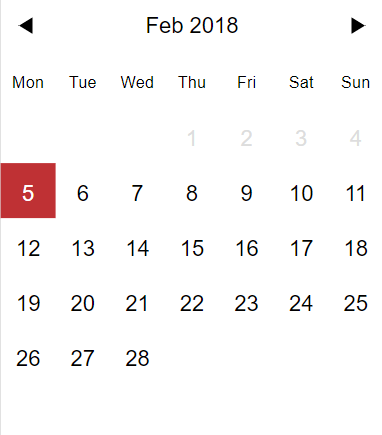
\includegraphics[width=0.6\linewidth]{images/date-picker}
		\caption{Date picker}
		\label{fig:date-picker}
	\end{subfigure}
	\begin{subfigure}[b]{0.48\textwidth}
		\centering
		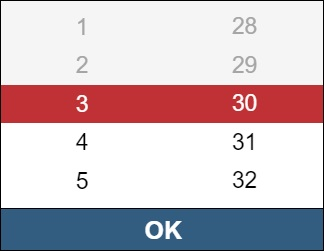
\includegraphics[width=0.6\linewidth]{images/time-picker}
			\caption{Time picker}
		\label{fig:time-picker}
	\end{subfigure}
	\caption[Date picker a Time picker]{}
\end{figure}


\subsection{Zobrazovanie zastávok na mape}
Aplikácia ponúka možnosť výberu zastávky priamo z mapy v prípade, že používateľ nepozná názvy zastávok. Na prácu s mapou používame knižnicu $vue-google-maps$. Po zvolení možnosti zadania zastávky z mapy, vycentruje pohľad mapy na aktuálnu polohu používateľa. 

Najskôr sme zobraziť všetky existujúce zastávky naraz. Bežné mobilné zariadenie však nestíhalo prekresľovať obrazovku pri posúvaní pohľadu z dôvodu hustého rozsadenia zastávok. Bolo potrebné optimalizovať zobrazenie zastávok. 

Ďalej sme zvažovali sme zobrazovanie zastávok rovnakým spôsobom ako ich zobrazuje aplikácia $Google Maps$, a to tak, že používateľ vidí zastávky len ak je dostatočne priblížený. V prípade, že používateľ vidí celú Bratislavu, nevidí žiadne zastávky. 

Nakoniec sme zobrazovanie zastávok vyriešili tak, že zastávky sa budú zobrazovať len v určitom výreze $V$, ktorý je centrovaný v strede obrazovky. Tento výrez $V$ bude obdĺžnikového tvaru a jeho veľkosť sa bude z pohľadu používateľa meniť podľa hodnoty priblíženia pohľadu. 
Pri každej zmene hodnoty priblíženia pohľadu, získame súradnice hraničných bodov zobrazenej plochy. Pomocou získaných súradníc, vypočítame reálnu rozlohu ohraničenej plochy $S$. Zvolili sme si konštantu $k$, ktorá určuje maximálnu rozlohu výrezu $V$. 
Ak je $S > k$, zastávky zobrazíme zastávky vo výreze $V$ s rozlohou $k$, ako môžeme vidieť na obrázku \ref{fig:map-view} (a) a (b). Z pohľadu používateľa je rozloha výrezu V na obrázkoch rôzna, avšak v skutočnosti je rozloha rovnaká, pretože sa jedná o reálnu rozlohu.
Ak je $S < k$, tak zastávky zobrazím na celej obrazovke ako môžeme vidieť na obrázku \ref{fig:map-view}(c). V tomto prípade je dokonca $k > V$.

\begin{figure}[H]
\centerline{\includegraphics[width=0.8\textwidth]{images/map-view}}
\caption[Zobrazenie zastávok na mape]{Zobrazenie zastávok na mape}
\label{fig:map-view}
\end{figure}

\subsection{Zobrazovanie časov ciest}
Pri vypisovaní jednotlivých ciest na klientskej strane sme sa museli viackrát zamyslieť, ako zobraziť meškanie vozidla. Najskôr sme sa inšpirovali aplikáciami, ktoré tiež zobrazujú meškania spojov. Vypísali sme pri zastávke na nastúpenie a pri zastávke na vystúpenie časy príchodov podľa statických cestovných poriadkov. K tomu sme pripísali aj informáciu o meškaní prípadne nemeškaní spoja. Používateľ by si však musel sám prepočítať, kedy má spoj predpokladaný príchod v prípade meškania. MHD spoje často meškajú a používateľ by často musel prepočítavať. To nie je veľmi používateľsky prívetivé. Ukážka zobrazenia je na onrázku \ref{fig:time-view-bad1}.

Ďalšou možnosťou je zobraziť oba časy – čas podľa statických cestovných poriadkov a aj ten s pripomínaným omeškaním. Ako môžeme vidieť na obrázku \ref{fig:time-view-bad2} toto riešenie pôsobí chaoticky, pretože na jednej stránke je zobrazených príliš veľa časov. 

\begin{figure}[H]
\centering
	\begin{subfigure}[b]{0.48\textwidth}
		\centering
 		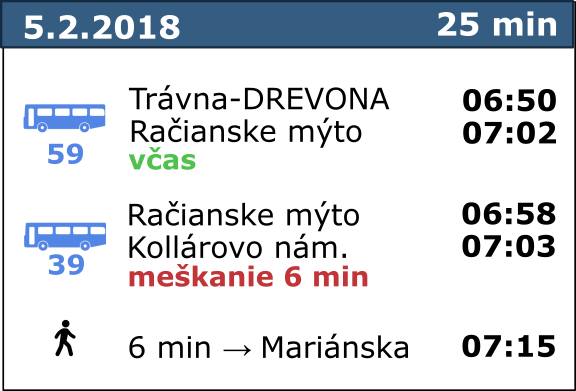
\includegraphics[width=0.7\linewidth]{images/time-view1}
		\caption{ }
		\label{fig:time-view-bad1}
	\end{subfigure}
	\begin{subfigure}[b]{0.48\textwidth}
		\centering
		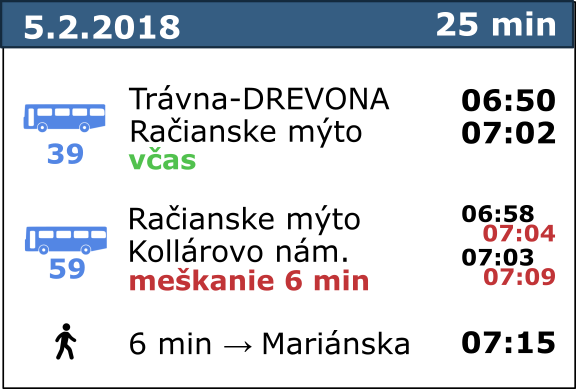
\includegraphics[width=0.7\linewidth]{images/time-view2}
			\caption{ }
		\label{fig:time-view-bad2}
	\end{subfigure}
	\caption[Možnosti zobrazenia časov v ceste]{Možnosti zobrazenia časov v ceste}
\end{figure}

Rozhodli sme sa tento problém vyriešiť tak, že budeme zobrazovať len pripočítaný čas, ktorý udáva, kedy má spoj príchod na zastávku podľa statických cestovných poriadkov s pripočítaným predpokladaným meškaním. Časy spoja budú označené farebne. V prípade, že vozidlo už vyrazilo a nemá žiadne meškanie, časy budú zafarbené zelenou farbou. Meškajúce spoje budú mať červené časy a spoje, ktoré ešte nevyrazili budú mať časy čierne. 
Po kliknutí na cestu sa zobrazí detail cesty, kde je pri každej zastávke zobrazený čas zo statických cestovných  poriadkov a pri spoji je zobrazený stav meškania. Zobrazenie cesty aj detail cesty je zobrazený na obrázku \ref{fig:time-view-good}.


\begin{figure}[H]
\centering
	\begin{subfigure}[b]{0.48\textwidth}
		\centering
 		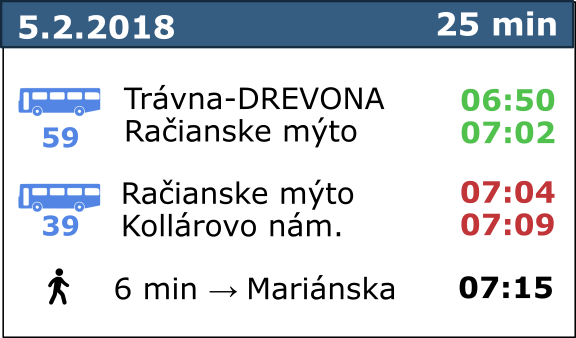
\includegraphics[width=0.7\linewidth]{images/time-view3}
	\end{subfigure}
	\begin{subfigure}[b]{0.48\textwidth}
		\centering
		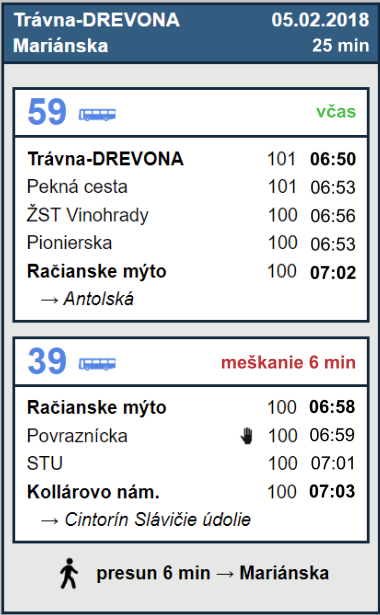
\includegraphics[width=0.7\linewidth]{images/time-view-detail}
	\end{subfigure}
	\caption[Finálne zobrazenie časov v ceste]{Finálne zobrazenie časov v ceste}
	\label{fig:time-view-good}
\end{figure}

\subsection{Nasledujúce cesty}
Pre vyhľadanie optimálnych ciest používateľ zadáva povinné vstupné parametre: začiatočnú a konečnú zastávku, dátum a čas $\tau$. Ostatné parametre sú dobrovoľné a sú predvolené. Klient si vždy uloží posledné vyhľadávané parametre do stavu a pošle dopyt na server. Ako odpoveď  dostane aspoň $x$ ciest, ktoré nezačínajú skôr ako čas $\tau$. Server sa teda stará o to, aby bol dostatočný počet ciest na jednu stránku. V prípade, že používateľ chce nasledujúce cesty, pod poslednou vyhľadanou cestou sa nachádza tlačidlo "Nasledujúce". Kliknutím na toto tlačidlo klient pripočíta k času odchodu poslednej cesty jednu minútu. Následne pošle dopyt so zapamätanými vyhľadávacími parametrami na server s tým, že zmení čas prípadne aj dátum. 




























